\documentclass[a4paper]{article}
\usepackage{ctex}
\usepackage[left=1.5cm, right=1.5cm, top=1.5cm, bottom=1.5cm]{geometry} %页边距
\usepackage{helvet}
\usepackage{amsmath, amsfonts, amssymb} % 数学公式、符号
\usepackage[english]{babel}
\usepackage{graphicx}   % 图片
\usepackage{url}        % 超链接
\usepackage{bm}         % 加粗方程字体
\usepackage{multirow}
\usepackage{booktabs}
\usepackage{tikz}%调用宏包tikz
\usepackage{circuitikz}%调用宏包circuitikz
\usepackage{enumerate}
\usepackage{algorithm}
\usepackage{algorithmicx}
\usepackage{algpseudocode}
\usepackage{graphicx}
\usepackage[hidelinks]{hyperref}
\usepackage{listings}
\usepackage{textcomp}
\usepackage{multicol}
\usepackage[backend=biber,style=numeric,sorting=none]{biblatex}
\addbibresource{reference.bib}

% Python listing
\newcommand\pythonstyle{\lstset{
language=Python,
basicstyle=\sffamily,
keywordstyle=\textbf,
commentstyle=\color{blue},
showstringspaces=false, 
numbers=left }}
% Python environment
\lstnewenvironment{python}[1][]{
\pythonstyle \lstset{#1} }{}

\newcommand{\threemetrics}[3]{\multirow{3}{*}{\shortstack[c]{$\textcolor{orange}{#1}$\\$\textcolor{blue}{#2}$\\$\textcolor{green}{#3}$}}}
\newcommand{\twometrics}[2]{\multirow{2}{*}{\shortstack[c]{$\textcolor{blue}{#1}$\\$\textcolor{green}{#2}$}}}

\renewcommand{\algorithmicrequire}{ \textbf{Input:}}       
\renewcommand{\algorithmicensure}{ \textbf{Output:}} 
%算法格式
\usepackage{subfigure}
\usepackage{fancyhdr} %设置页眉、页脚
\usepackage{gensymb}

\pagestyle{fancy}
\lhead{Computer Architecture, Homework2}
\chead{}
\rhead{2024,Lab2}
\lfoot{}
\cfoot{\thepage}
\rfoot{All experiments please refer to the assembly codes.}


\usepackage{ifthen}
\usepackage{xifthen}

\newcommand{\dom}[1]{\mathop{\mathrm{dom}}\left(#1\right)}
\newcommand{\rng}[1]{\mathop{\mathrm{rng}}\left(#1\right)}
\newcommand{\preimg}[2][]{ \ifthenelse{\isempty{#1}}
    {\mathop{\mathrm{preimage}}\left(#2\right)}
    {\mathop{\mathrm{preimage}}_{#1}\left(#2\right)} }
\newcommand{\set}[1]{\left\{#1\right\}}

\newenvironment{proof}{{\par\noindent\it Proof.}\quad\par}{\hfill $\square$\par}  


\begin{document}
    \section{Explanation of the code}
    \subsection{Module}
    The module operation is applied as follows. Assuming A mod B. \\
    $\bullet$ 1. Using the POP and PUSH mechanisms showed in the textbook.\\
    $\bullet$ 2. For positive number, we store A into the register, and keep subtracting B from A.
    When A becomes negative, instead of storing A to register, we extract the value stored inside the register
    and store it directly to R0. Then we display it.\\
    $\bullet$ 3. For negative number, we keep adding B to A until it become a positive number, then we store it into
    R0. Then we display it.
    \subsection{XOR}
    For XOR operation, we have:\\
    $\bullet$ 1. We extract each bit by started at 1, and each time after extract 1 bit, we left shift it after 
    using it to clear the carries produced by ADD operation to extract next bit.\\
    $\bullet$ 2. Then, After we extract the bit, we applied ADD operation to get XOR value on that bit.\\
    $\bullet$ 3. Don't forget to use the bit extractor (in bullet 1) to clear the carries. Then left shift the bit extractor.
    \subsection{Other explaination}
    \noindent
    $\bullet$ 1. Remember that the PCoffset in LC3 is only [-256,255]. So when some label is out of range,
    we can create other symbol and using `.FILL' instruction to get the symbol that is out of range. For LEA 
    some symbols which are out of range, use `.FILL' and LD instead of LEA.\\
    $\bullet$ 2. The code of POP part in second edition is wrong, for R6 was pointing at the ``Bottom'' of the stackBase and 
    when checking in POP function, the R0 is pointing at the stackBase. So we should modify the `BRz Underflow' to `BRp Underflow'.
    An alternative way is to delete `ADD R0,R0,\#1', which is adopted by 3rd edition.\\
    \section{The result of the code}
    \begin{figure}[H]
        \centering  %图片全局居中
        \subfigure[ADD]{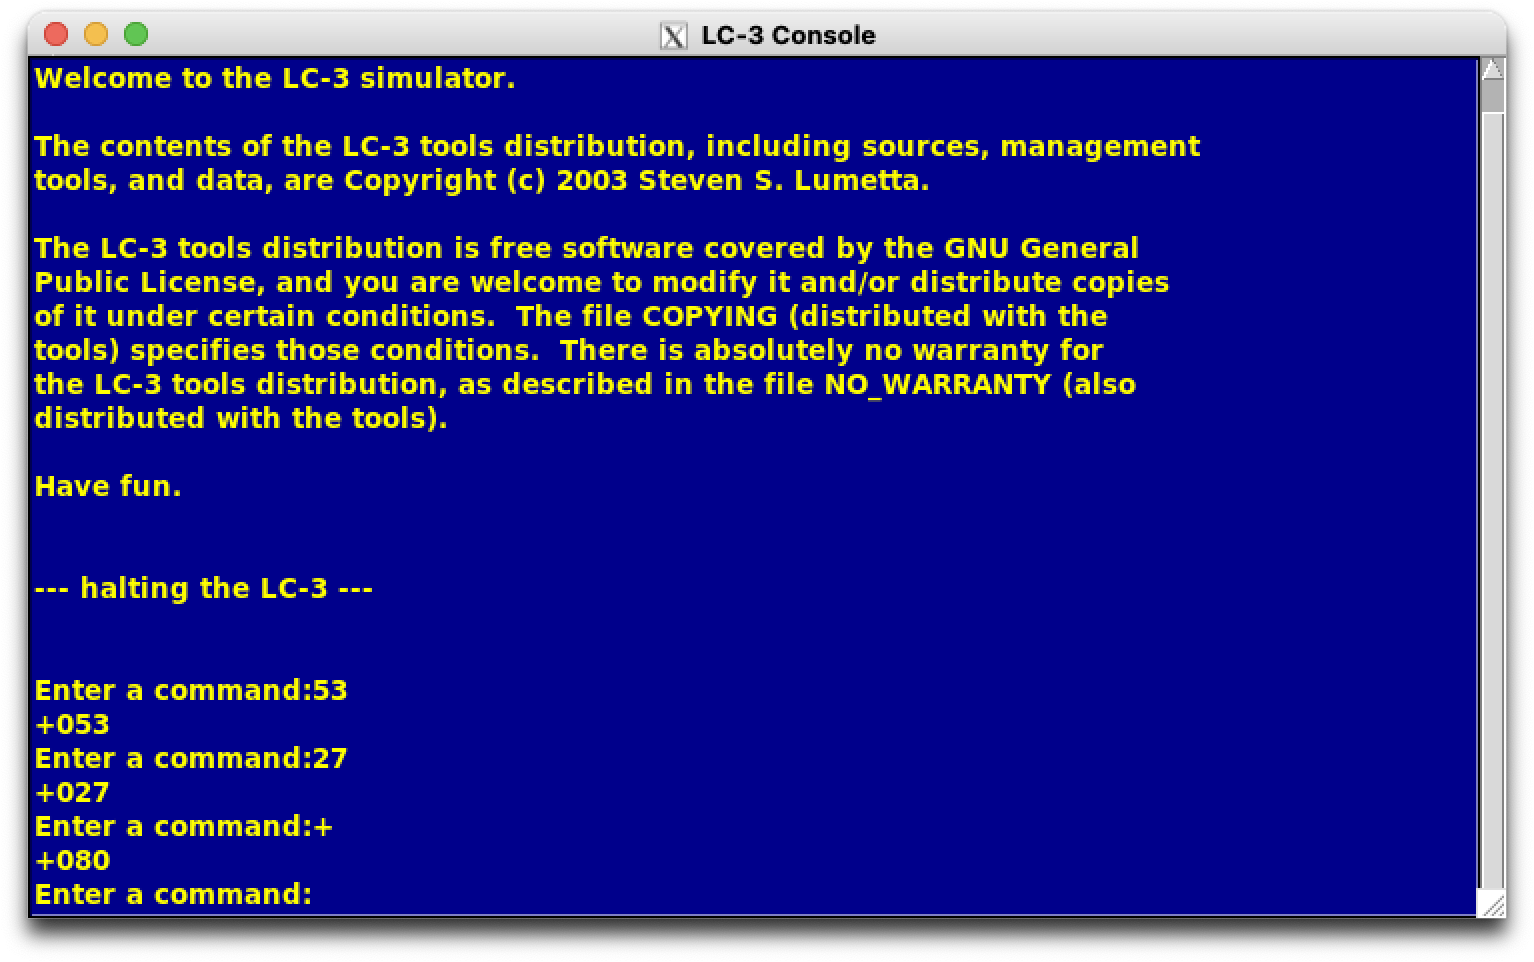
\includegraphics[scale=0.16]{1.png}}
        \subfigure[MINUS]{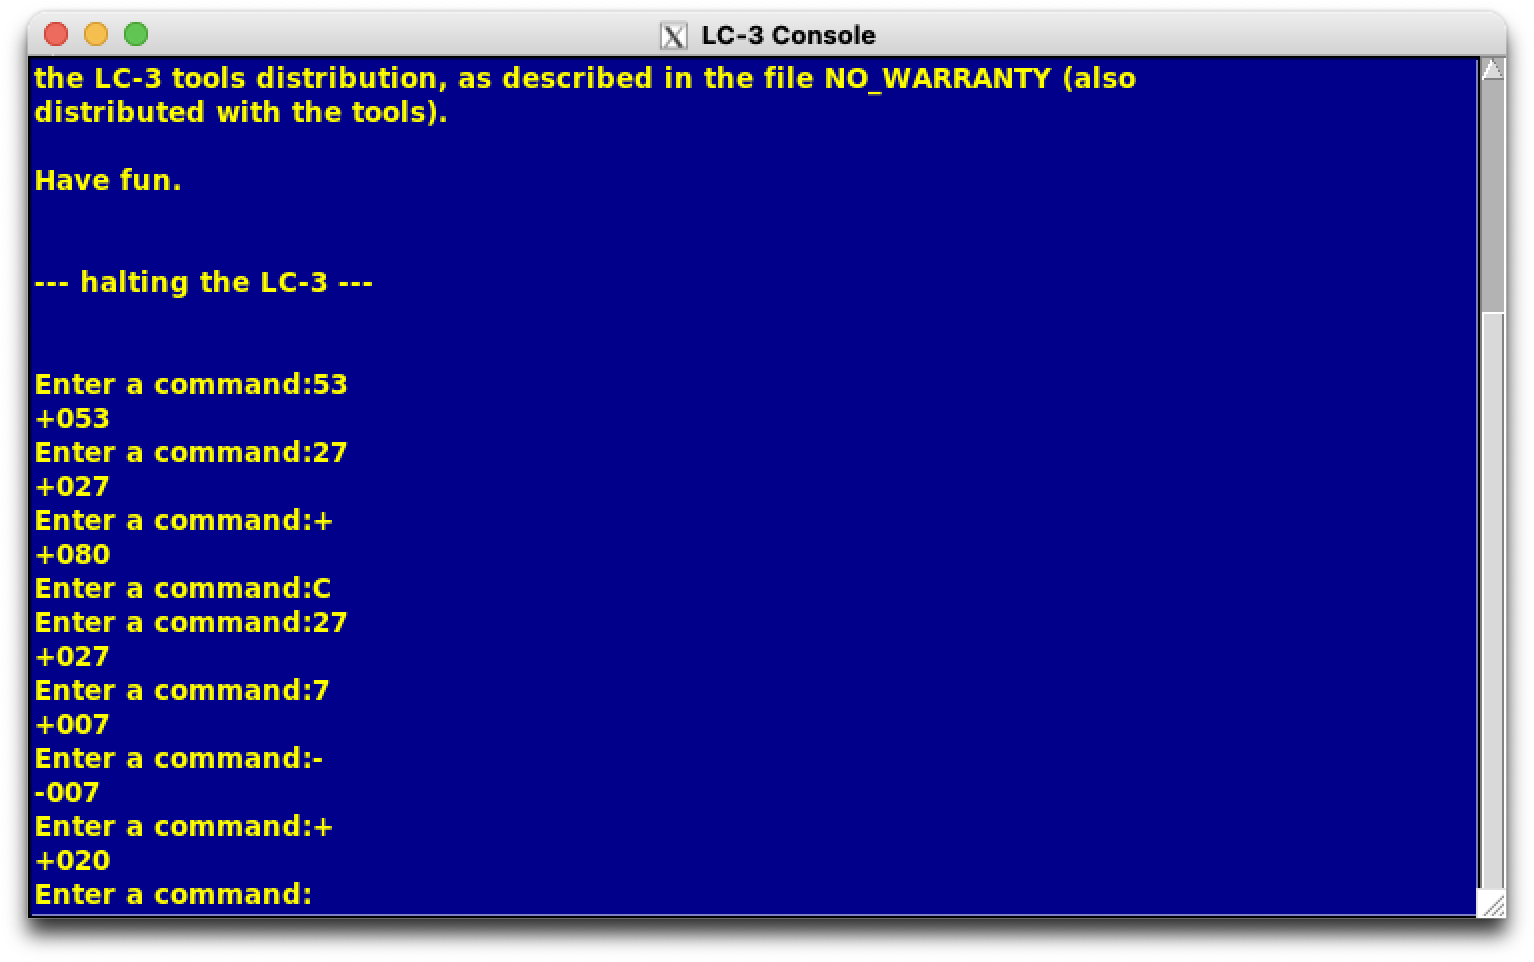
\includegraphics[scale=0.16]{2.png}}
    \end{figure}
    \begin{figure}[H]
        \centering
        \subfigure[MULTIPLY]{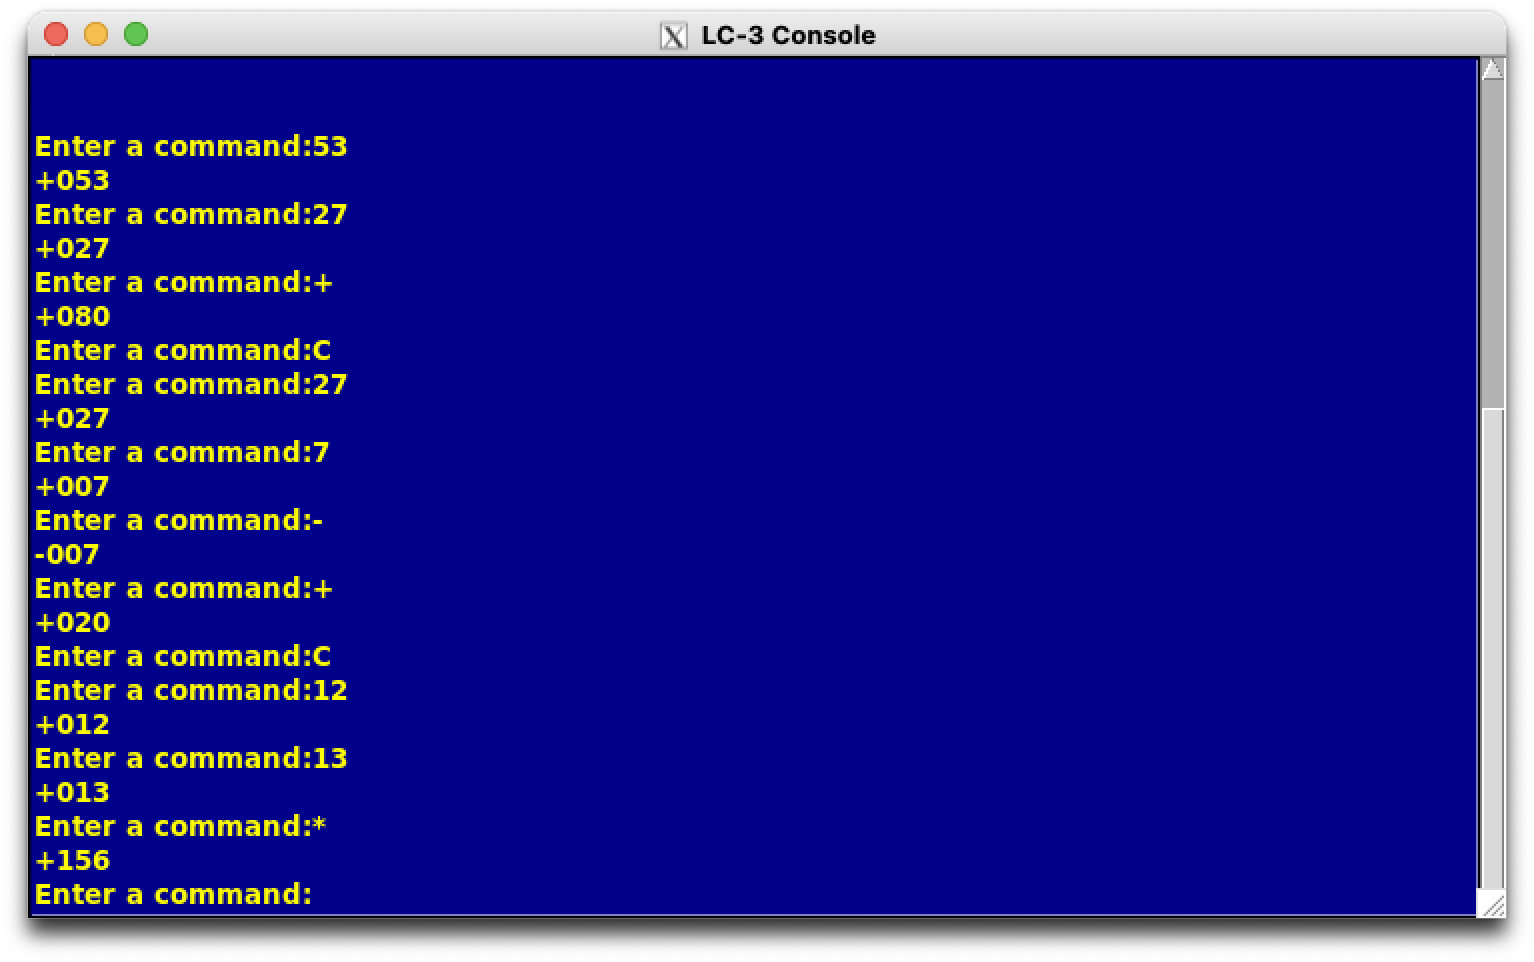
\includegraphics[scale=0.16]{3.png}}
        \subfigure[XOR]{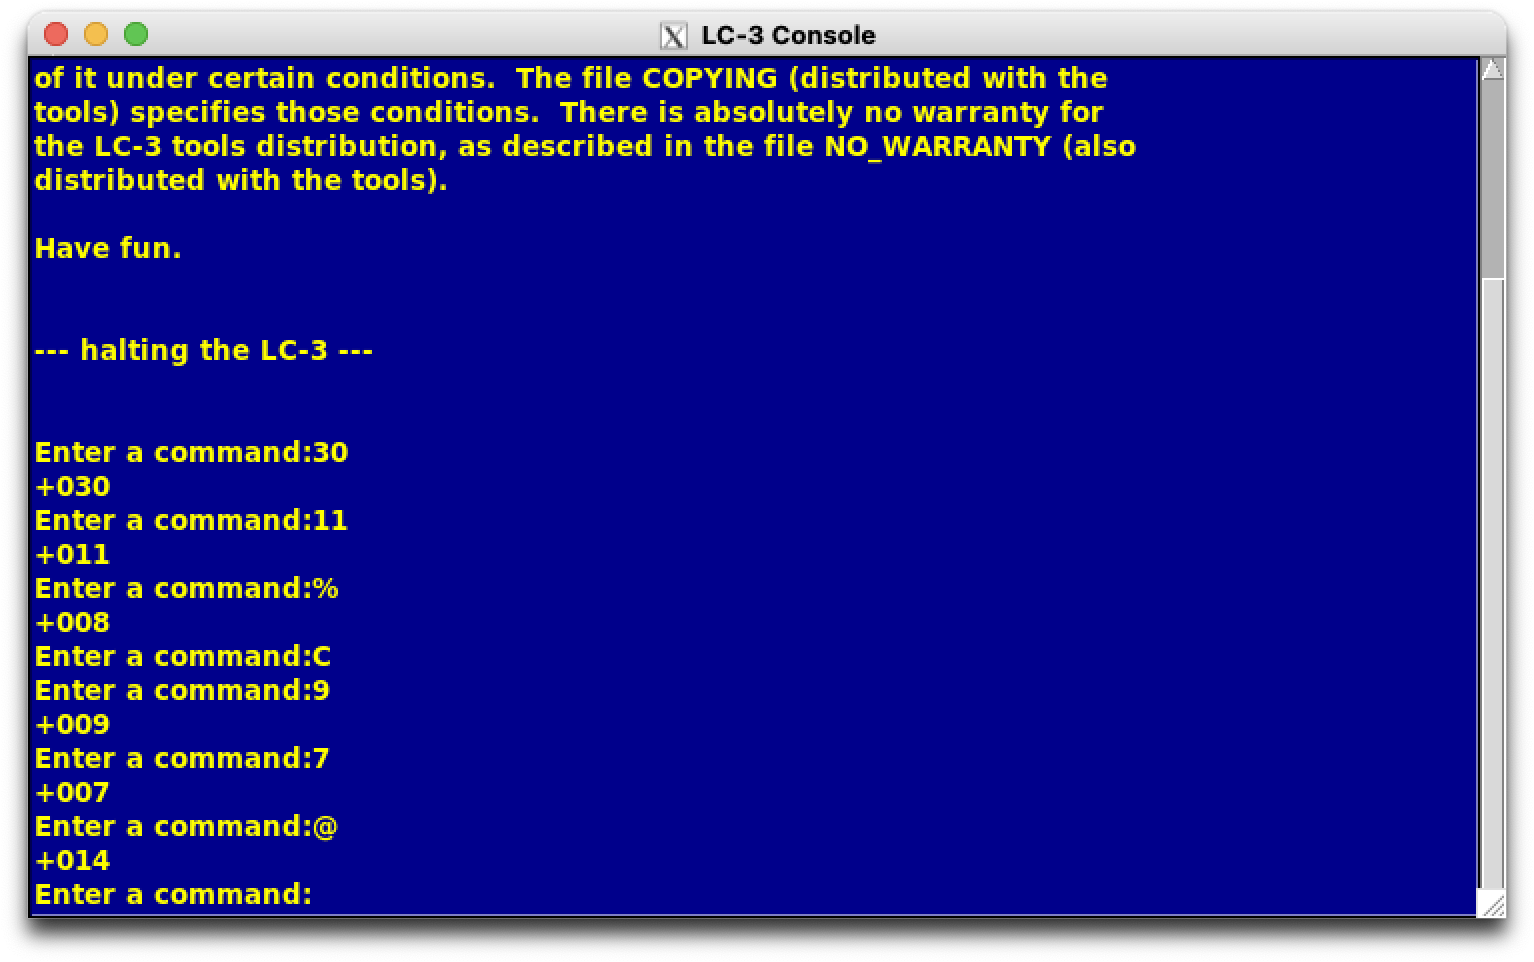
\includegraphics[scale=0.16]{5.png}}
        \subfigure[POSITIVE MOD]{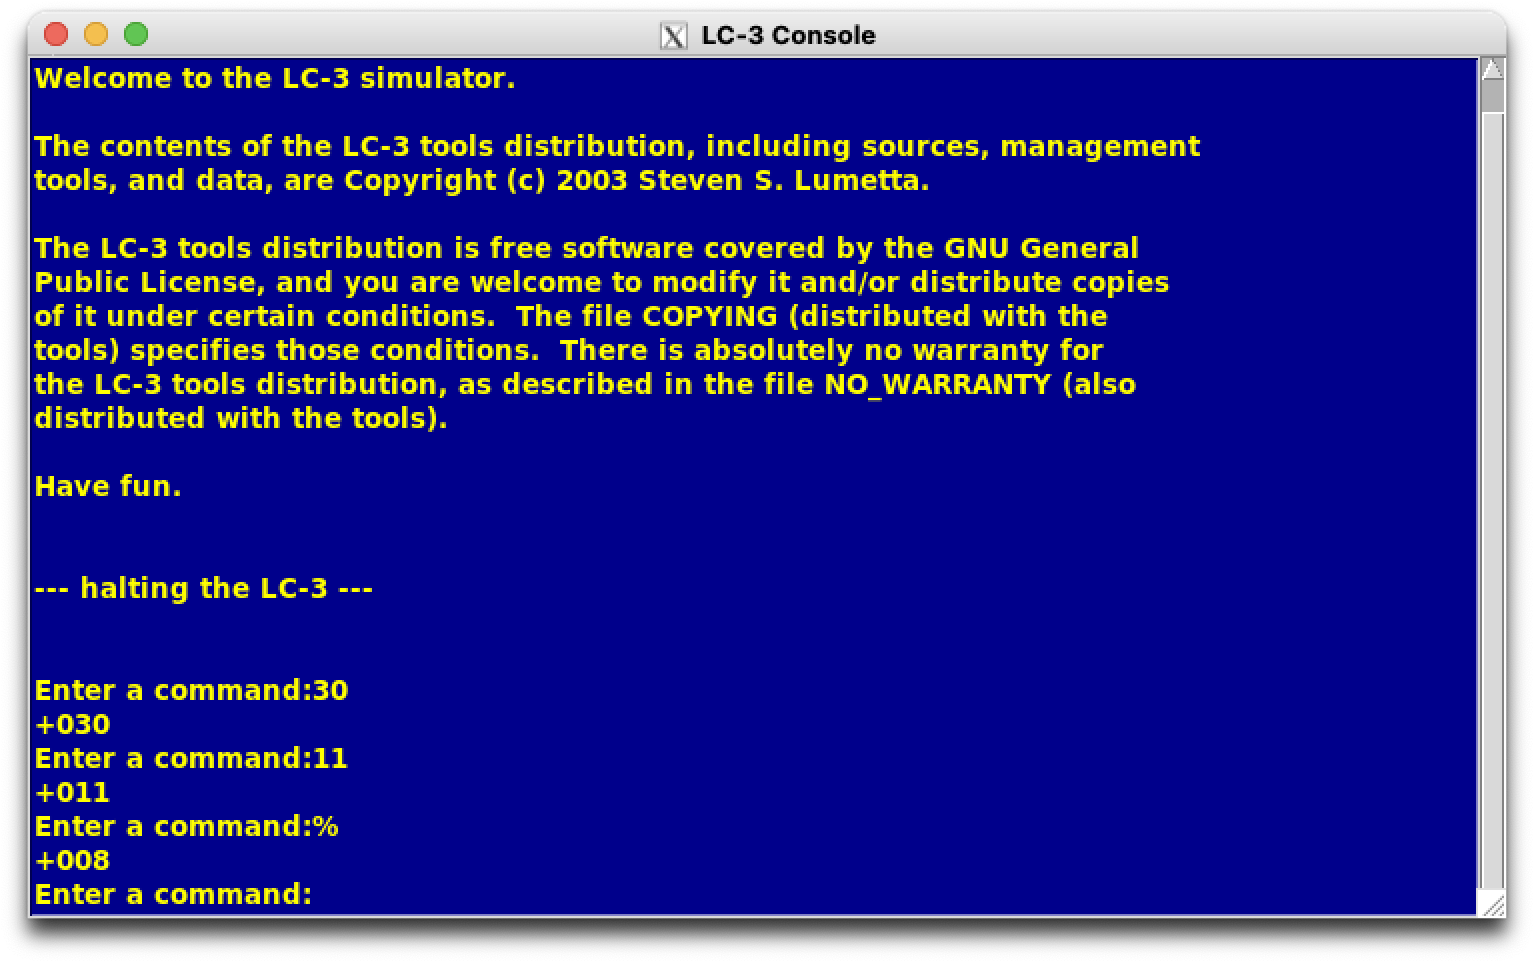
\includegraphics[scale=0.16]{4.png}}
        \subfigure[NEGATIVE MOD]{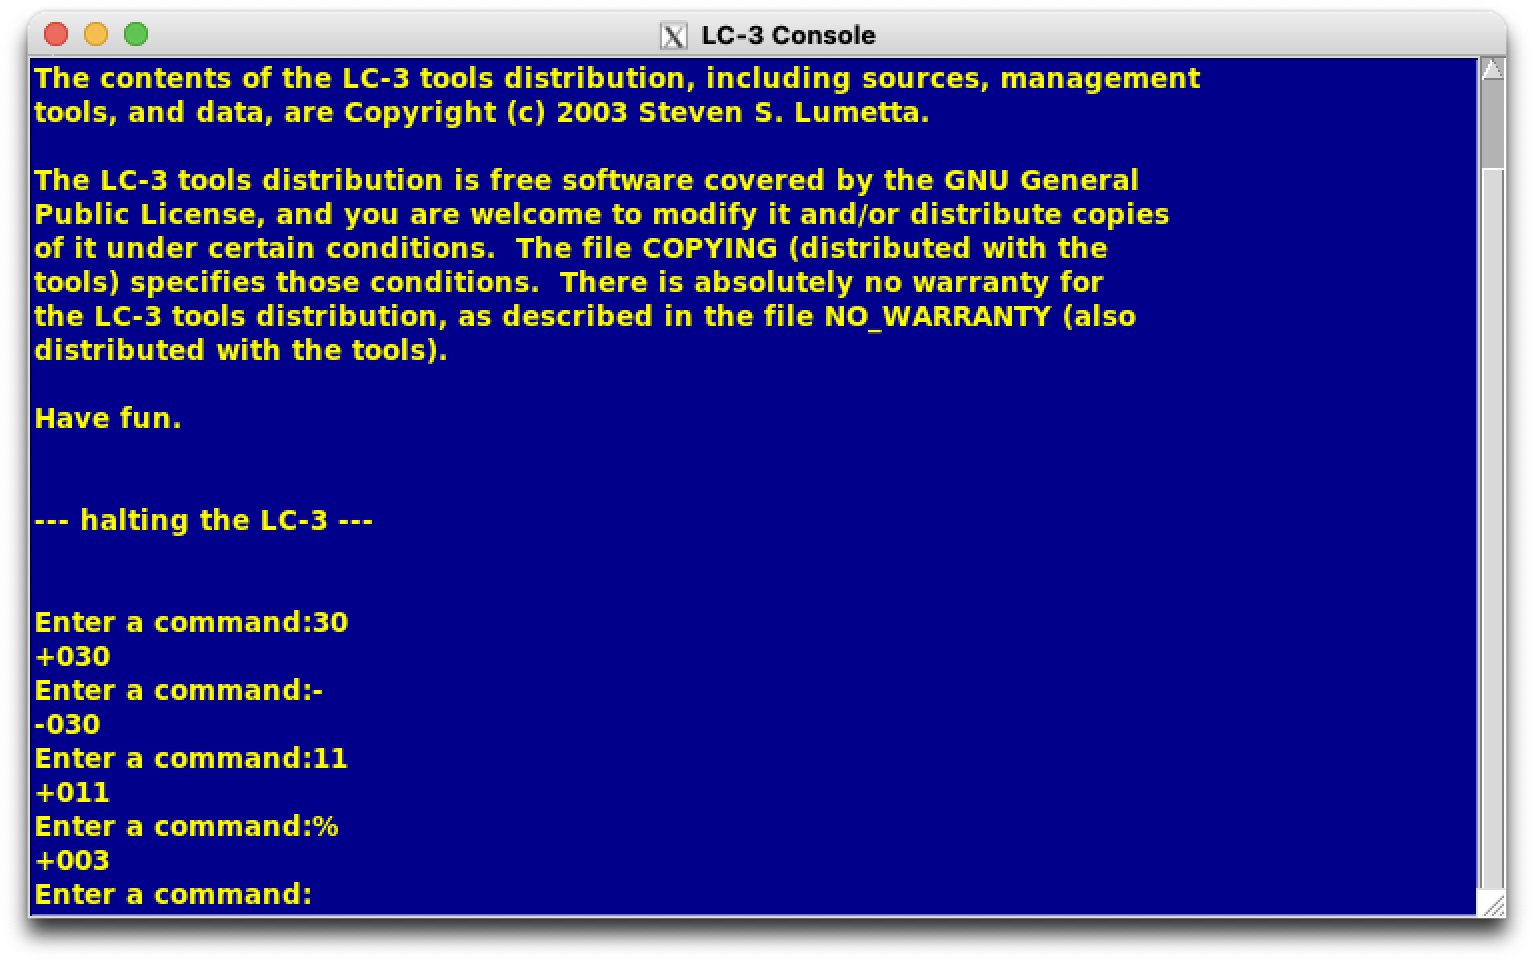
\includegraphics[scale=0.16]{8.png}}
        \subfigure[DISPLAY]{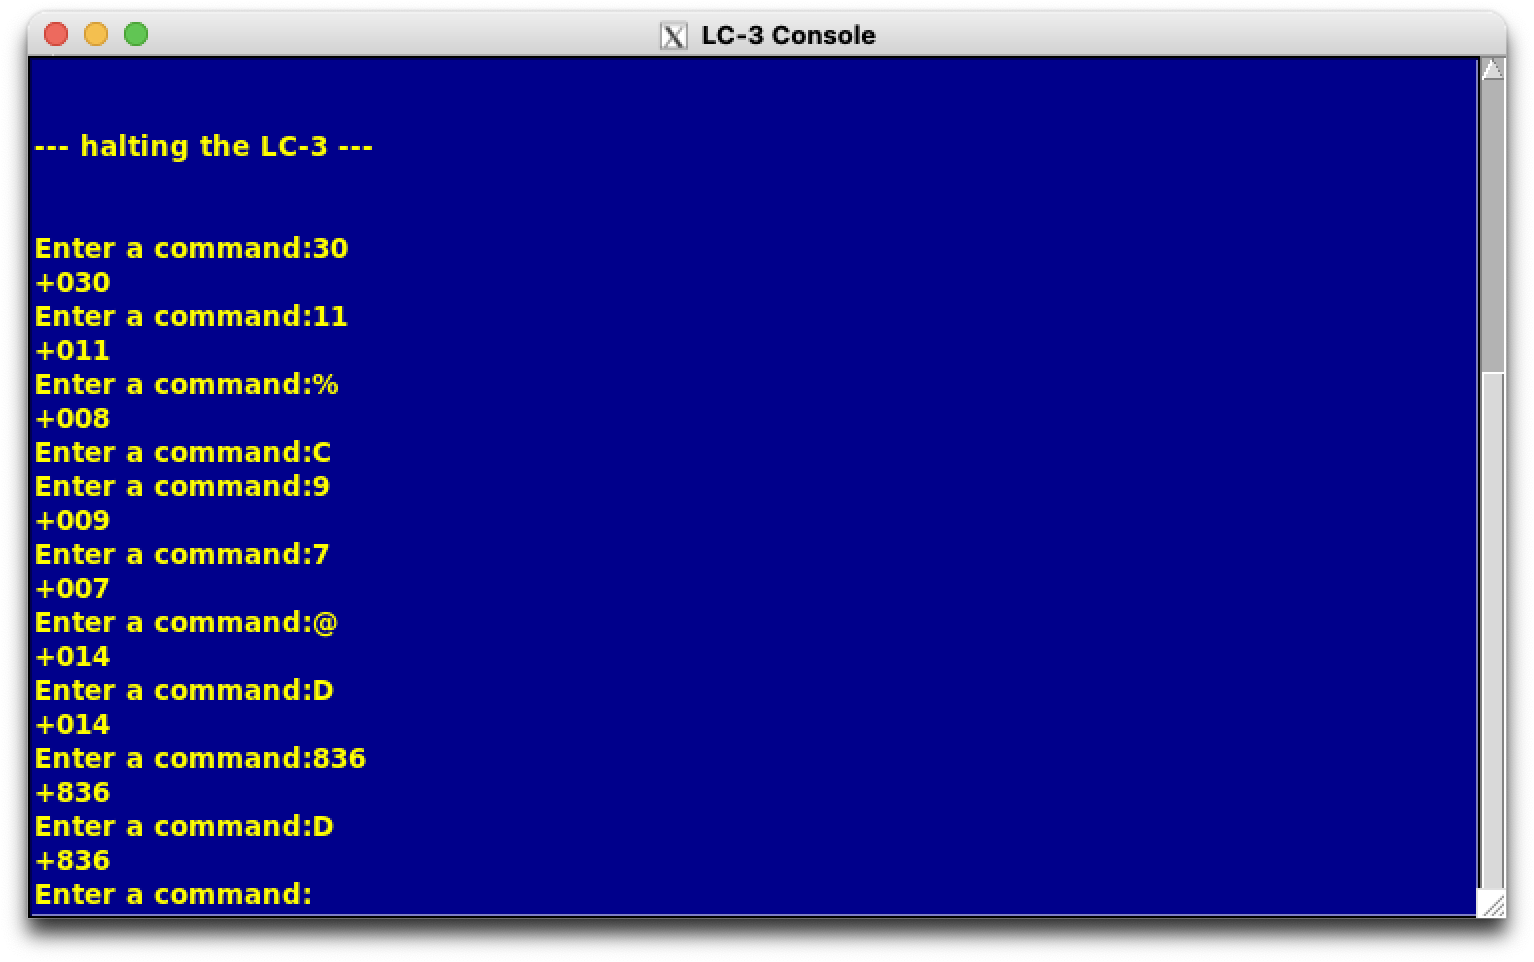
\includegraphics[scale=0.16]{6.png}}
        \subfigure[EXIT]{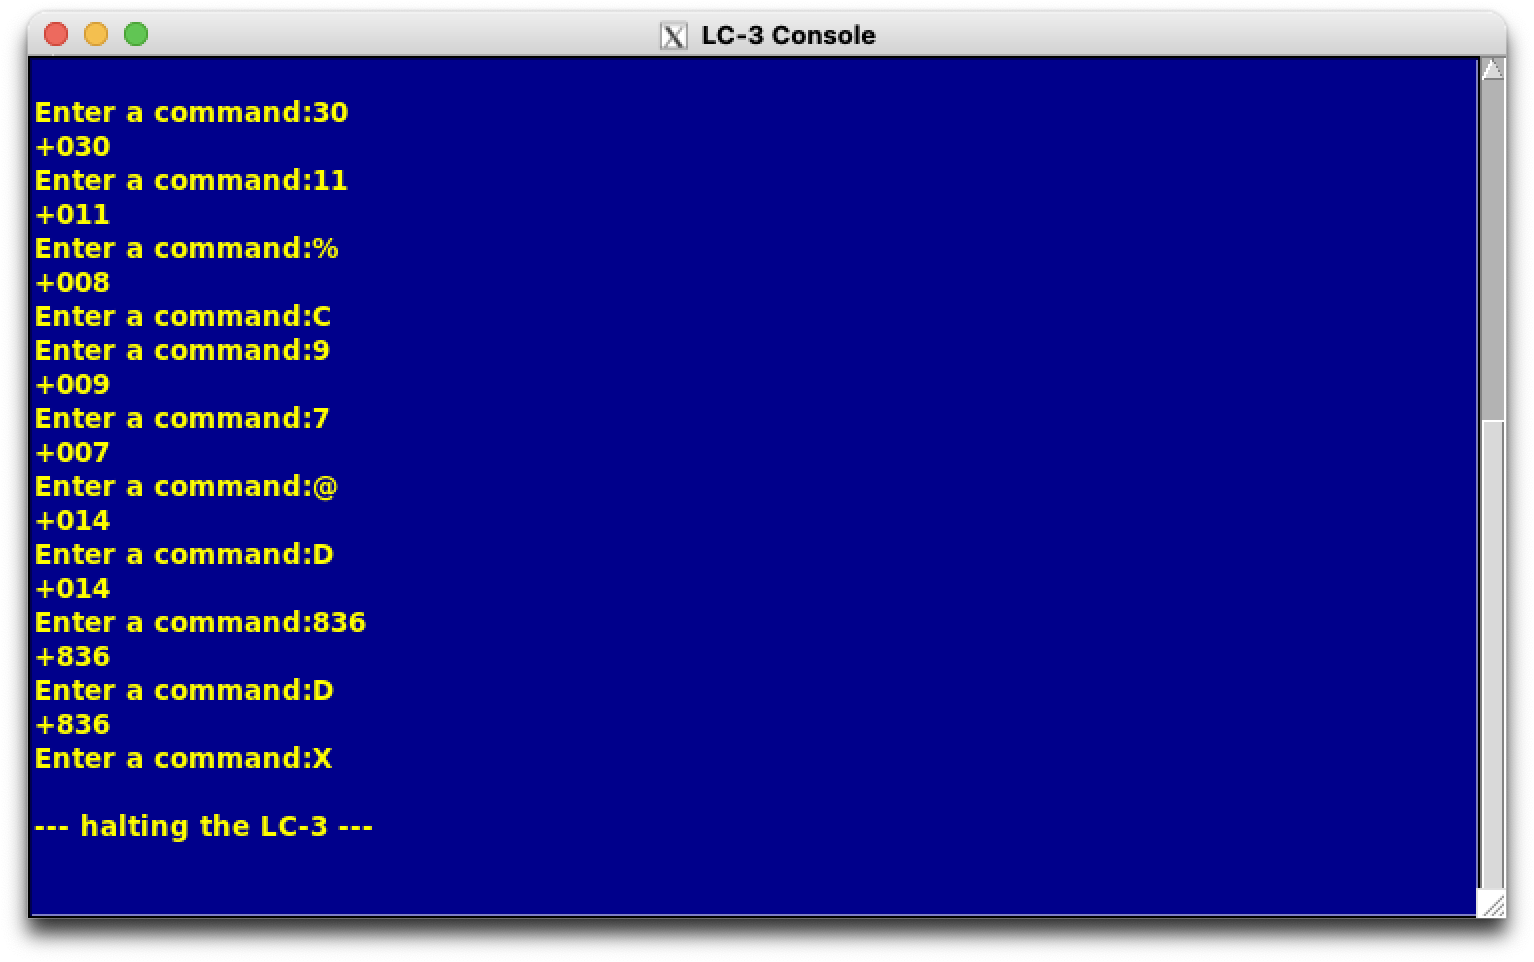
\includegraphics[scale=0.16]{7.png}}
    \end{figure}
\end{document}